 \documentclass[
11pt, % The default document font size, options: 10pt, 11pt, 12pt
% codirector, % Uncomment to add a codirector to the title page
]{charter} 


% El títulos de la memoria, se usa en la carátula y se puede usar el cualquier lugar del documento con el comando \ttitle
\titulo{Implementación de un sistema de bootloader para el circuito integrado SiWG917} 

% Nombre del posgrado, se usa en la carátula y se puede usar el cualquier lugar del documento con el comando \degreename
\posgrado{Carrera de Especialización en Sistemas Embebidos} 
%\posgrado{Carrera de Especialización en Internet de las Cosas} 
%\posgrado{Carrera de Especialización en Inteligencia Artificial}
%\posgrado{Maestría en Sistemas Embebidos} 
%\posgrado{Maestría en Internet de las cosas}
% IMPORTANTE: no omitir titulaciones ni tildación en los nombres, también se recomienda escribir los nombres completos (tal cual los tienen en su documento)
% Tu nombre, se puede usar el cualquier lugar del documento con el comando \authorname
\autor{Ing. Guido Ramírez}

% El nombre del director y co-director, se puede usar el cualquier lugar del documento con el comando \supname y \cosupname y \pertesupname y \pertecosupname
\director{Esp. Ing. Jonathan Cagua}
\pertenenciaDirector{Easymetering} 
\codirector{} % para que aparezca en la portada se debe descomentar la opción codirector en los parámetros de documentclass
\pertenenciaCoDirector{FIUBA}

% Nombre del cliente, quien va a aprobar los resultados del proyecto, se puede usar con el comando \clientename y \empclientename
\cliente{Joffre Anzules}
\empresaCliente{Easymetering}
 
\fechaINICIO{20 de agosto de 2024}		%Fecha de inicio de la cursada de GdP \fechaInicioName
\fechaFINALPlan{8 de octubre de 2024} 	%Fecha de final de cursada de GdP
\fechaFINALTrabajo{15 de junio de 2025}	%Fecha de defensa pública del trabajo final


\begin{document}

\maketitle
\thispagestyle{empty}
\pagebreak


\thispagestyle{empty}
{\setlength{\parskip}{0pt}
\tableofcontents{}
}
\pagebreak


\section*{Registros de cambios}
\label{sec:registro}


\begin{table}[ht]
\label{tab:registro}
\centering
\begin{tabularx}{\linewidth}{@{}|c|X|c|@{}}
\hline
\rowcolor[HTML]{C0C0C0} 
Revisión & \multicolumn{1}{c|}{\cellcolor[HTML]{C0C0C0}Detalles de los cambios realizados} & Fecha      \\ \hline
0      & Creación del documento                                 &\fechaInicioName \\ \hline
1      & Se completa hasta el punto 5                & 3 de septiembre de 2024 \\ \hline
2      & Se completa hasta el punto 9 & 10 de septiembre de 2024 \\ \hline
3      & Se completa hasta el punto 12                & 17 de septiembre de 2024 \\ \hline
4      & Se completa el plan	                                 & 23 de septiembre de 2024 \\ \hline

% Si hay más correcciones pasada la versión 4 también se deben especificar acá

\end{tabularx}
\end{table}

\pagebreak



\section*{Acta de constitución del proyecto}
\label{sec:acta}

\begin{flushright}
Buenos Aires, \fechaInicioName
\end{flushright}

\vspace{2cm}

Por medio de la presente se acuerda con el \authorname\hspace{1px} que su Trabajo Final de la \degreename\hspace{1px} se titulará ``\ttitle'' y consistirá en la integración del equipo mencionado a un sistema de producción por medio de un arrancador génerico, portable y escalable. El trabajo tendrá un presupuesto preliminar estimado de 628 horas y un costo estimado de \$9855, con fecha de inicio el \fechaInicioName\hspace{1px} y fecha de presentación pública el \fechaFinalName.

Se adjunta a esta acta la planificación inicial.

\vfill

% Esta parte se construye sola con la información que hayan cargado en el preámbulo del documento y no debe modificarla
\begin{table}[ht]
\centering
\begin{tabular}{ccc}
\begin{tabular}[c]{@{}c@{}}Dr. Ing. Ariel Lutenberg \\ Director posgrado FIUBA\end{tabular} & \hspace{2cm} & \begin{tabular}[c]{@{}c@{}}\clientename \\ \empclientename \end{tabular} \vspace{2.5cm} \\ 
\multicolumn{3}{c}{\begin{tabular}[c]{@{}c@{}} \supname \\ Director del Trabajo Final\end{tabular}} \vspace{2.5cm} \\
\end{tabular}
\end{table}




\section{1. Descripción técnica-conceptual del proyecto a realizar}
\label{sec:descripcion}

\section{1.1 Estado del arte}
\label{sec:estadoDelArte}

\section{1.1.1 Bootloader}
\label{sec:edaBootloader}

Un bootloader o arrancador no es diferente a una aplicación cómun en un microcontrolador. De hecho, es igual a una aplicación común. Lo que hace especial a este es su propósito: permitir la actualización y administración de software sin usar un hardware especializado, y en algunos casos, ser el primer punto de chequeo de integridad de un sistema embebido. Existen variedad de bootloaders; pueden comunicarse a través de diferentes protocolos como UART, CAN, I2C, Ethernet, USB, entre otros. Los sistemas que poseen un arrancador tienen dentro dos programas coexistiendo y deben ser capaces de detectar la existencia de actualizaciones de sistema en progreso.

Cada boootloader puede tener requerimientos únicos basados en su aplicación objetivo, sin embargo existen procesos generales como la capacidad de cambiar entre programa y bootloader, comunicación a través de una interfaz, análisis de registros, guardado de datos en memoria no vólatil, chequeo de integridad de aplicaciones y seguridad del código almacenado. Independientemente de los requerimientos de la aplicación, los procesos generales inducen a una operación relativamente estandar.

En la figura \ref{fig:bootloaderFlow} se puede observar la operación de un bootloader génerico. Se destaca que en el incio del programa se decide ejecutar la aplicación o al arrancador. Este último tiene la capacidad de receptar y ejectuar comandos, y finalmente salir de la aplicación. Los comandos abarcan las operaciones generales mencionadas anteriormente, y pueden añadir el uso de otros periféricos o el envio de datos adicionales hacia un anfitrión.

\begin{figure}[htpb]
\centering 
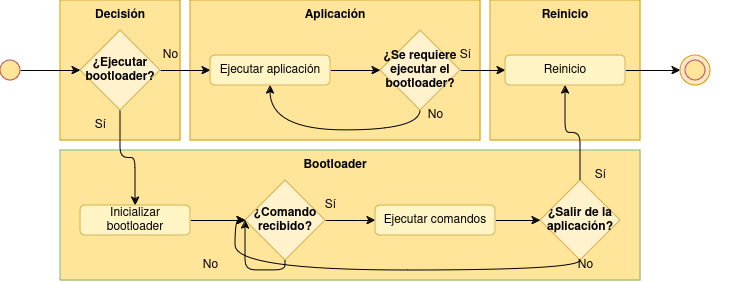
\includegraphics[width=.99\textwidth]{./Figuras/GdP-diagrams-bootloader.png}
\caption{Operación génerica de un bootloader.}
\label{fig:bootloaderFlow}
\end{figure}

\newpage

\section{1.2 Problemática}
\label{sec:s1Problematica}

Easymetering es una empresa que diseña y distribuye módulos AMI (Advanced Metering Infraestructure por sus siglas en inglés). Los módulos AMI son sistemas que miden, recolectan y analizan el uso de la energía, e interactúan con dispositivos como los medidores inteligentes de electricidad, de gas o de agua. Estos son capaces de gestionar información recolectada y tomar deciciones.

Actualmente, ofrecen productos basados en los microcontroladores de los fabricantes Nordic, Microchip, NXP y Espressif. Los módulos AMI, solución más vendida en América latina, usan microcontroladores del último fabricante. Por otro lado, productos usando otras familias se producen o se venden muy poco  .La compañía, con visión de ingresar a otros mercados, ha decidido ampliar su cartera de productos incorporando familias de microcontroladores basados en procesadores ARM Cortex-M a sus módulos AMI. Una de las ventajas de esto, es su escalabilidad, es decir, no se limitan a microcontroladores de bajo costo, sino que los fabricantes han diseñado una serie de soluciones a distintas necesidades. Entre ellas destacan microcontroladores con multiples proccesadores para procesamiento extensivo de señales digitales o datos; sistemas integrados en un chip (SoC por sus siglas en inglés) para manejo de energía, sistemas de control, conectividad e internet de las cosas.

Agregar nuevos microcontroladores a la solución AMI de Easymetering, conlleva incorporarlo a su sistema de producción. Este se encarga de guardar información relevante del módulo como seriales del equipo, interfaces de red y periféricos. Actualmente, existe un arrancador o binario de producción que no contempla la inclusión de nuevas familias de microcontroladores y su implementación es bastante específica para microcontroladores de Espressif. También, existen distintas versiones de arrancador específicos para otras familias. Esto dificulta la incorpración de nuevas solciones o requisitos.  Por ende, se plantea desarrollar un arrancador génerico y portable.

\section{1.3 Solución}
\label{sec:s1Solución}

En el diagrama de descomposición de la figura \ref{fig:sec1BootloaderSolution} se muestra la comunicación entre los módulos para el bootloader génerico propuesto. A pesar de que los procesos generales mostrados al principio de la sección no están explicitamente mencionados, serán considerados en la propuesta. El bootloader será capaz de interactuar con el sistema de producción de la compañía, receptando y ejecutando comandos. Es importante destacar que los módulos a realizar seguirán buenas prácticas de programación, lo que resultará en escalabilidad y portabilidad. 

\begin{figure}[htpb]
\centering 
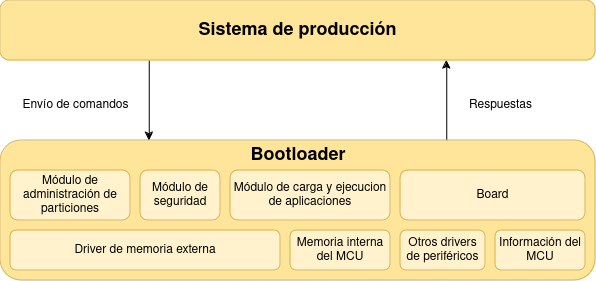
\includegraphics[width=.65\textwidth]{./Figuras/GdPDiagrams-sec1_solution.png}
\caption{Diagrama de descomposición para bootloader propuesto.}
\label{fig:sec1BootloaderSolution}
\end{figure}

Los módulos de administración de particiones, seguridad y carga y ejecución de aplicaciones juegan un rol importante para el bootloader. Son los encargados de interactuar con la memoria externa usada e interna del microcontrolador. Las interacciones con la primera son son leer, escribir y borrar aplicaciones. La relación con la memoria del microcontrolador consiste en escribir aplicaciones provenientes de la otra memoria y ejecutarlas cuando se requiera. Por otro lado, el módulo de administración de particiones y seguridad se encargará de dividir la memoria externa y establecer parámetros de seguridad para chequear la integridad de sus contenidos. Por último, el módulo de \textit{board} interactua cercanamente con la información proporcionada por \textit{drivers} de otros periféricos y del microcontrolador, con la finalidad de enviar datos relevantes al sistema de producción.

El valor agregado de la propuesta es un bootloader reutilizable y escalable para futuras soluciones que usen otras familias de microcontroladores. Además, cumple con la necesidad específica de la compañía de incorporar un sistema de almacenamiento de binarios propio, con particionamiento y lineamientos de seguridad personalizados.

\newpage

\section{2. Identificación y análisis de los interesados}
\label{sec:interesados}

\begin{table}[ht]
%\caption{Identificación de los interesados}
%\label{tab:interesados}
\begin{tabularx}{\linewidth}{@{}|l|X|X|l|@{}}
\hline
\rowcolor[HTML]{C0C0C0} 
Rol           & Nombre y Apellido & Organización 	& Puesto 	\\ \hline
Cliente       & \clientename      &\empclientename	&    Gerente General    \\ \hline
Responsable   & \authorname       & FIUBA        	& Alumno 	\\ \hline
Orientador    & \supname	      & \pertesupname 	& Director del Trabajo Final \\ \hline
Usuario final & Departamento de firmware/producción & Easymetering &       - 	\\ \hline
\end{tabularx}
\end{table}

\begin{itemize}
	\item Orientador: el \supname\  tiene una larga trayectoria como desarrollador de firmware y hardware. Tiene experiencia usando varios microcontroladores incluyendo el seleccionado para este proyecto.
\end{itemize}

\section{3. Propósito del proyecto}
\label{sec:proposito}


El próposito del proyecto es desarrollar un \textit{bootloader} portable para distintas familias de microcontroladores, inicialmente dirigido hacia el SoC SiWG917. El proyecto nace de la integración de nuevos productos basados en otras familias de microprocesadores con el objetivo de ofrecerlos e implementarlos en otros mercados. El \textit{bootloader} debe acoplarse al sistema de producción actual de la compañía. El arrancador usa una memoria externa particionada con lineamientos de seguridad establecidos por el cliente; almacena y administra aplicaciones binarias. Además, se comunica con el sistema de producción a través de una computadora anfitriona para ejecutar comandos y almacenar datos relevantes del equipo. 

\section{4. Alcance del proyecto}
\label{sec:alcance}

El proyecto incluye:
\begin{itemize}
	\item Desarrollo del driver para el manejo de memoria flash externa.
	\item Diseño de particiones de la memoria flash externa.
	\item Manejo de archivos \textit{linker} del microcontrolador.
	\item Integración de capas de seguridad en las imágenes del dispositivo.
	\item Integración con el sistema de producción de la empresa
		\begin{itemize}
		\item Comunicación serial.
		\item Control de versiones de hardware.
		\item Control de versiones de firmware.
		\item Control de inventario.
		\end{itemize}	
\end{itemize}

El proyecto no incluye:
\begin{itemize}
	\item Diseño de hardware.
	\item Comunicación Wi-Fi con el sistema de producción.
\end{itemize}

\section{5. Supuestos del proyecto}
\label{sec:supuestos}

Para el desarrollo del presente proyecto se supone que:

\begin{itemize}
	\item Existencias dentro de la compañía del integrado \textit{W25Q64JVZPIQTR}, memoria flash externa.
	\item Disponibilidad de una placa de desarrollo basada en el SoC objetivo.
	\item Una computadora para el desarrollo del proyecto.
	\item Disponibilidad del equipo de backend para consultas sobre el sistema de producción.
	\item Un equipo de software estará disponible para la integración del nuevo SoC en la base de datos del sistema de producción.
\end{itemize}

\section{6. Requerimientos}
\label{sec:requerimientos}

\begin{enumerate}
	\item Requerimientos funcionales:
		\begin{enumerate}
			
			\item La placa debe acoplarse al sistema de producción de la empresa.
			\item La placa debe guardar los datos de producción de la compañía.
			\item El usuario puede cargar distintos binarios a la placa objetivo.
			\item El usuario puede arrancar cualquier binario cargado a la placa objetivo.
			\item El sistema debe poder volver al bootloader.
			\item El sistema detecta cuándo hubo una actualización de binarios.
			\item Los binarios almacenados no son guardados en texto plano.
			\item Los binarios, antes de ser almacenados, son encriptados usando el módulo de seguridad del sistema.
		\end{enumerate}
	\item Requerimientos de documentación:
		\begin{enumerate}
			\item Documentación usando Doxygen en todos los módulos, componentes o drivers.
			\item Redacción de la planificación del proyecto.
			\item Redacción de la memoria técnica.
		\end{enumerate}
	\item Requerimiento de testing:
		\begin{enumerate}
			\item Testing de driver para memoria externa.
			\item Testing de driver para consola.
			\item Testing de administración de particiones.
			\item Testing de módulo de seguridad.
			\item Testing de componente board.
		\end{enumerate}
	\item Requerimientos de la interfaz:
		\begin{enumerate}
			\item Imitar el sistema de producción para prueba de concepto.
		\end{enumerate}
\end{enumerate}

\section{7. Historias de usuarios (\textit{Product backlog})}
\label{sec:backlog}

A continuación, se dan a conocer historias de usarios valoradas con \textit{story points}, basados en tres categorías aplicadas en cada historia: dificultad, D; complejidad, C; y riesgo, R. Cada categoría tiene asignada tres niveles: bajo, medio y alto. Cada nivel es asociado con un puntaje de 1, 2 y 3 respectivamente. Finalmente, se suman los niveles asignados a cada categoría para obtener la valoración final de la historia. Si la valoración no es un número de la serie Fibonacci, entonces se aproxima al número superior más cercano de la secuencia. El resultado nos informa de la dificultad, complejidad y riesgo del trabajo a realizar para cada historia de usuario.

\begin{itemize}
	\item ``Como miembro del departamento de firmware, espero que el bootloader de nuestros equipos sea escalable para incorporar nuevas tecnologías o requerimientos, con la finalidad de trabajar o dar mantenimiento a un único proyecto de softwar''
	\begin{itemize}
		\item D:3 + C:3 + R:2 $\rightarrow$ 8
	\end{itemize}
	\item ``Como miembro del departamento de firmware, aspiro a tener un sistema de arranque y administración de binarios genérico, para mantener nuestro código reutilizable y escalable"
	\begin{itemize}
		\item D:3 + C:2 + R:1 $\rightarrow$ 8
	\end{itemize}
	\item ``Como encargado del departamento de producción, me interesa que nuevos productos sean incorporados fácilmente en nuestra base de datos, para minimizar el tiempo empleado en cada orden"
	\begin{itemize}
		\item D:2 + C:2 + R:1 $\rightarrow$ 5
	\end{itemize}
	\item ``Como encargado del departamento de producción, quiero manejar una única versión actualizada de bootloader, para poder cargar binarios de aplicación para distintas soluciones o productos."
	\begin{itemize}
		\item D:3 + C:3 + R:3 $\rightarrow$ 13
	\end{itemize}
	\item ``Como CEO de Easymetering, deseo a futuro delegar ordenes de producción grandes de nuestras soluciones a las fabricas ensambladoras, con un bootloader que siga nuestros lineamientos de seguridad y encriptación, para evitar la filtración de nuestros binarios de aplicación."
	\begin{itemize}
		\item D:1 + C:3 + R:3 $\rightarrow$ 8
	\end{itemize}
\end{itemize}

\section{8. Entregables principales del proyecto}
\label{sec:entregables}

Los entregables del proyecto son:

\begin{itemize}
	\item Documentación usando doxygen.
	\item Documentación de la partición de memoria externa usada.
	\item Diagrama de flujo de procesos relevantes.
	\item Código fuente del firmware para módulos, componentes o drivers.
	\item La placa objetivo es agregada al sistema de producción.
	\item Memoria del trabajo final.
\end{itemize}

\section{9. Desglose del trabajo en tareas}
\label{sec:wbs}

En esta sección se desglosa el trabajo a realizar en una lista de tareas generales y específicas. La implementación de módulos de software, en su mayoría, tiene una sub-tarea de \textit{Test Driven Development} (TDD) por sus siglas en inglés. Esta sub-item no debe confundirse con el de pruebas, la cual consiste en el uso de la placa objetivo para validar el funcionamiento del módulo.

\begin{enumerate}
\item Redacción de la planificación del proyecto (40 h).
	\begin{enumerate}
	\item Redacción del documento (40 h).	
	\end{enumerate} 
\item Familiarizarse con el kit de desarrollo del SoC (84 h).
	\begin{enumerate}
	\item Leer datasheets del SoC (4 h).
	\item Leer guias para desarrolladores del IDE (8 h).
	\item Familiarizarse con el IDE (24 h).
	\item Familiarizarse con el SDK del fabricante (24 h).
	\item Familiarizarse con el ambiente de configuración del fabricante (24 h).
	\end{enumerate}
\item Módulo de consola (32 h).
	\begin{enumerate}
	\item Diseño de módulo (8 h).
	\item Implementación de funciones (8 h).
	\item TDD (8 h).
	\item Pruebas (8 h).
	\end{enumerate}
\item Protocolo de sistema de producción (48 h).
	\begin{enumerate}
	\item Diseñar módulo para protocolo (8 h).
	\item Implementar funciones (24 h).
	\item TDD (8 h).
	\item Pruebas (8 h).
	\end{enumerate}
\item Driver memoria externa (44 h).
	\begin{enumerate}
	\item Leer documentación del integrado (4 h).
	\item Diseño del driver	(8 h).
	\item Implementación de funciones (16 h).
	\item TDD (8 h).
	\item Pruebas (8 h).
	\end{enumerate}
\item Módulo de seguridad (56 h).
	\begin{enumerate}
	\item Investigación de algoritmos usados en trabajos anteriores (8 h).
	\item Definir algoritmos a usar (8 h).
	\item Investigar librería de algoritmos disponible (8 h).
	\item Implementación de funciones (16 h).
	\item TDD (8 h).
	\item Pruebas (8 h).
	\end{enumerate}
\item Módulo de administración de particiones (80 h).
	\begin{enumerate}
	\item Investigación y diseño de control particiones (24 h).
	\item Diseño de cabecera para binarios (8 h).
	\item Diseño de información de producción guardada (8 h).
	\item Implementación de funciones (24 h).
	\item TDD  (8 h).
	\item Pruebas  (8 h).
	\end{enumerate}
\item Módulo de carga y ejecución de aplicaciones (92 h).
	\begin{enumerate}
	\item Investigar funcionamiento memoria en la palca (24 h).
	\item Diseño de módulo (24 h).
	\item Implementación de funciones (24 h).
	\item TDD (8 h).
	\item Pruebas (12 h).
	\end{enumerate}
\item Módulo de board (56 h).
	\begin{enumerate}
	\item Investigar módulos de board de otros fabricantes (8 h).
	\item Diseño del módulo (8 h).
	\item Implementación de funciones (24 h).
	\item TDD  (8 h).
	\item Pruebas  (8 h).
	\end{enumerate}
\item Redacción de memoria técnica (96 h).
	\begin{enumerate}
	\item Taller de trabajo final A (40 h).
	\item Taller de trabajo final B (40 h).
	\item Informe de avance  (8 h).
	\item Presentación final (8 h).
	\end{enumerate} 
\end{enumerate}

Cantidad total de horas: 628 h.

\newpage

\section{10. Diagrama de Activity On Node}
\label{sec:AoN}

En esta sección se presenta el diagrama de \textit{Activity on Node} en la figura \ref{fig:AoN} se observan varias tareas con dos tonos de colores. Las tareas de color amarillo son aquellas dirigidas a la escritura de documentos académicos necesarios para la culminación de la Carrera de Especialización de Sistemas Embebidos (CESE). Por otra parte, las azules son tareas enfocadas en investigación y desarrollo de la parte técnica del proyecto.

\begin{figure}[htpb]
\centering 
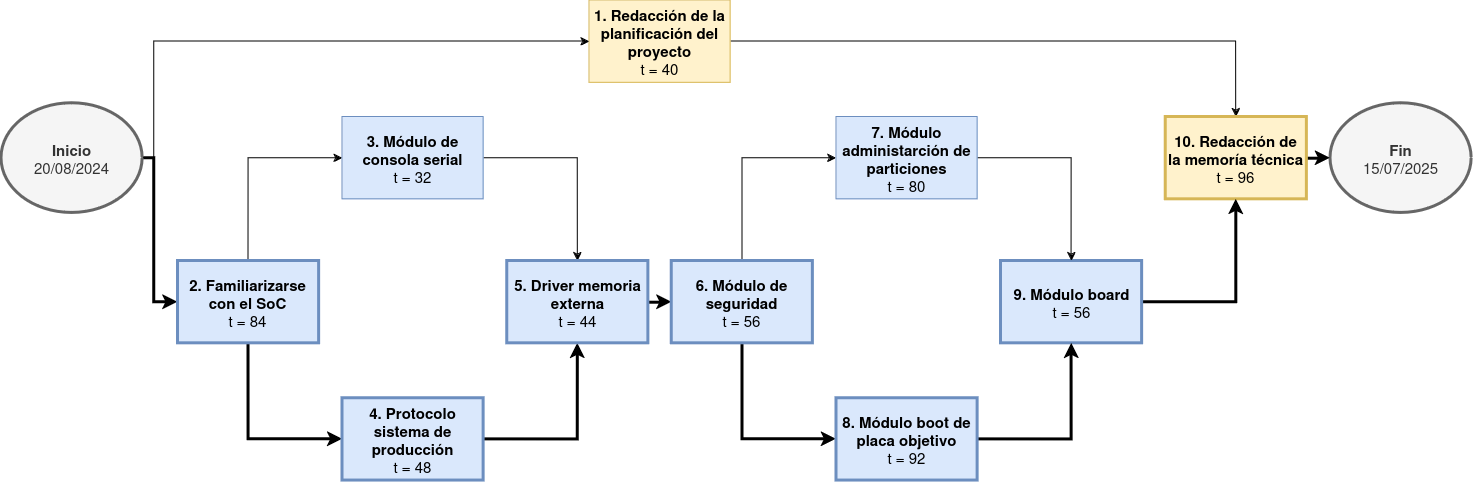
\includegraphics[width=1.0\textwidth]{./Figuras/GdPDiagrams-AoN_sec9.png}
\caption{Diagrama de \textit{Activity on Node}.}
\label{fig:AoN}
\end{figure}

En la figura también se puede distinguir el camino crítico del proyecto. La  unidad de los tiempos \textit{t} en el diagrama corresponde a horas. El camino crítico trazado toma 476 h. Se infiere por definición, que el retraso de cualquiera de las tareas parte del camino crítico llevará a una demora en todo el proyecto. Se puede notar que la actividades técnicas como la familarización con el SoC, implementación del driver de memoria externa, módulo de seguridad, arranque de placa objetivo y board forman parte de la ruta crítica y son parte de la propuesta de valor del proyecto. Por último, realizar la memoria técnica, necesaria para la culminiación de la especialización, es crítica dentro de las actividades desglosadas.

\section{11. Diagrama de Gantt}
\label{sec:gantt}

En el diagrama de Gantt mostrado en la figura \ref{fig:diagGantt} se puede apreciar de manera detallada la estructura de las tarea y sus dependencias. Se da a conocer una fecha estimada para la culminación del proyecto, la primera quincena de junio del 2025. 

\begin{landscape}
\begin{figure}[htpb]
\centering 
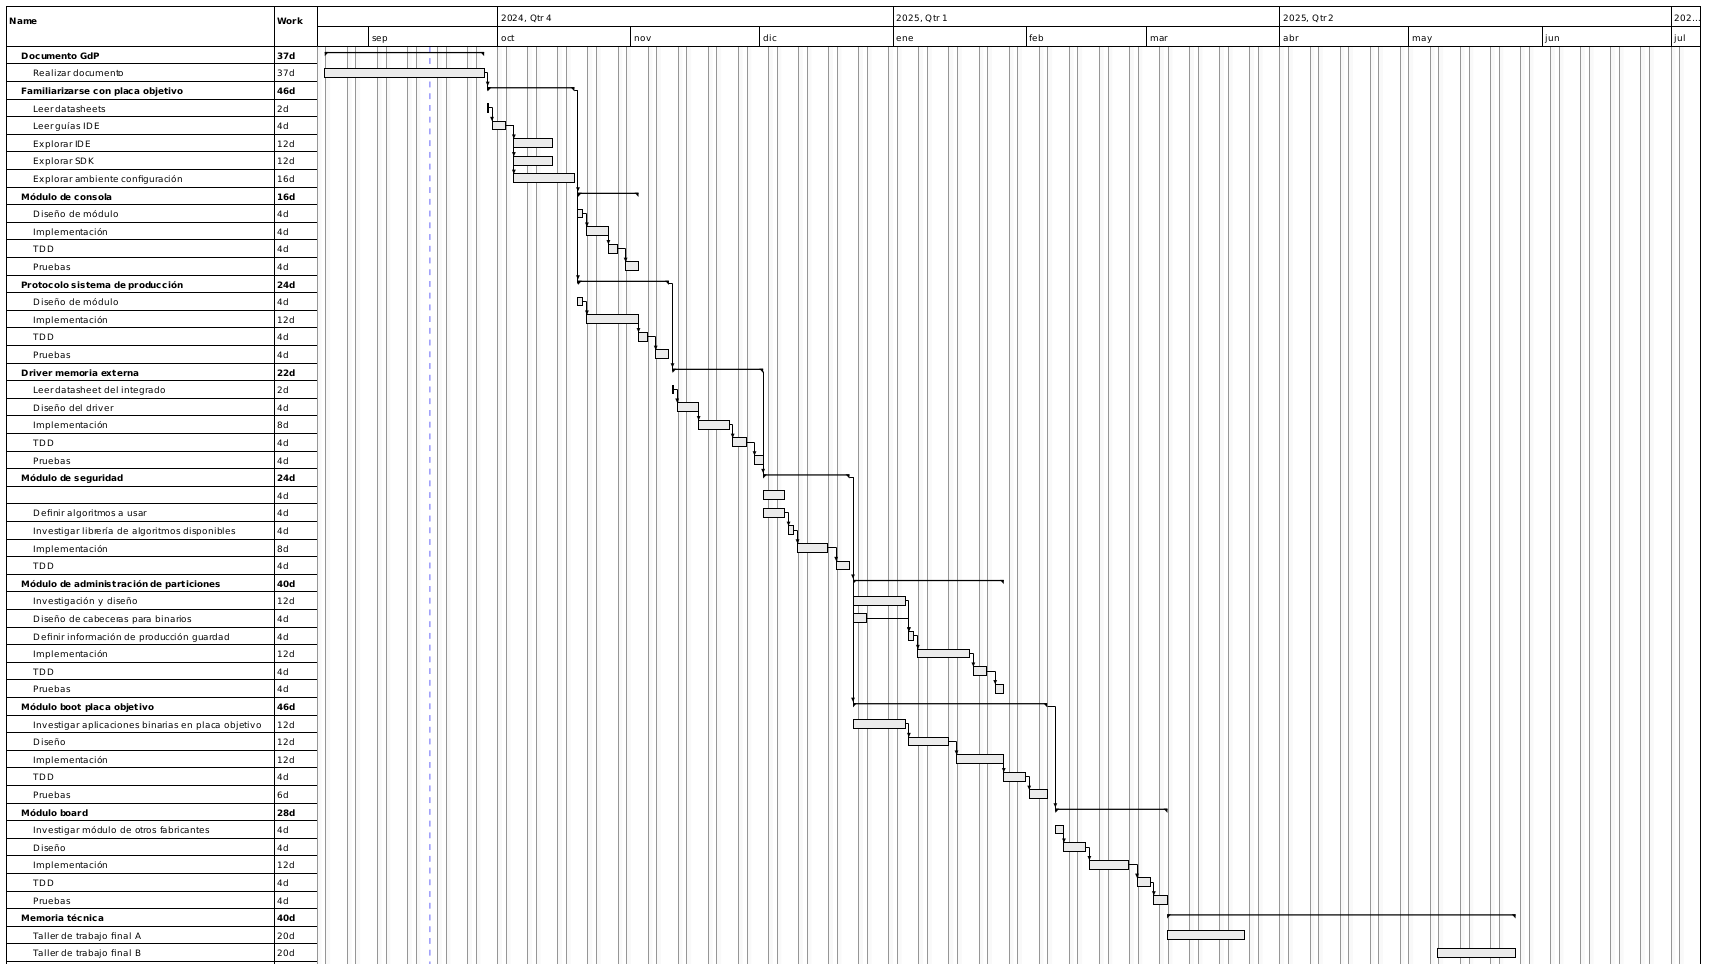
\includegraphics[height=.85\textheight]{./Figuras/Gdp-Gantt.png}
\caption{Planificación en diagrama de Gantt (apaisado).} %Modificar este título acorde.
\label{fig:diagGantt}
\end{figure}

\end{landscape}

\section{12. Presupuesto detallado del proyecto}
\label{sec:presupuesto}

En la tabla presentada en esta sección se puede ver el presupuesto detallado del proyecto dividido en costos directos e indirectos. La moneda usada es dólares (USD) y la tasa de conversión al día 15 de septiembre de 2024 es aproximadamente 960 ARS por USD.

\begin{table}[htpb]
\centering
\begin{tabularx}{\linewidth}{@{}|X|c|r|r|@{}}
\hline
\rowcolor[HTML]{C0C0C0} 
\multicolumn{4}{|c|}{\cellcolor[HTML]{C0C0C0}COSTOS DIRECTOS} \\ \hline
\rowcolor[HTML]{C0C0C0} 

  \multicolumn{1}{|l|}{Descripción} &
  \multicolumn{1}{c|}{\cellcolor[HTML]{C0C0C0}Cantidad} &
  \multicolumn{1}{c|}{\cellcolor[HTML]{C0C0C0}Valor unitario} &
  \multicolumn{1}{c|}{\cellcolor[HTML]{C0C0C0}Valor total} \\ \hline
  
  \multicolumn{1}{|l|}{Salario mensual} &
  \multicolumn{1}{c|}{6} &
  \multicolumn{1}{c|}{\$1250} &
  \multicolumn{1}{c|}{\$7500} \\ \hline

  \multicolumn{1}{|l|}{Módulo W25Q64 - 64 Mb / 8 MB - Adafruit } &
  \multicolumn{1}{c|}{1} &
  \multicolumn{1}{c|}{\$5.90} &
  \multicolumn{1}{c|}{\$5.90} \\ \hline
  
  \multicolumn{1}{|l|}{Placa de desarrollo SiWx917} &
  \multicolumn{1}{c|}{1} &
  \multicolumn{1}{c|}{\$100} &
  \multicolumn{1}{c|}{\$100} \\ \hline
  
\multicolumn{3}{|c|}{SUBTOTAL} &
  \multicolumn{1}{c|}{\$7605.90} \\ \hline
  
\rowcolor[HTML]{C0C0C0} 
\multicolumn{4}{|c|}{\cellcolor[HTML]{C0C0C0}COSTOS INDIRECTOS} \\ \hline
\rowcolor[HTML]{C0C0C0} 
Descripción &
  \multicolumn{1}{c|}{\cellcolor[HTML]{C0C0C0}Cantidad} &
  \multicolumn{1}{c|}{\cellcolor[HTML]{C0C0C0}Valor unitario} &
  \multicolumn{1}{c|}{\cellcolor[HTML]{C0C0C0}Valor total} \\ \hline
  
  \multicolumn{1}{|l|}{Laptop para desarrollo} &
  \multicolumn{1}{c|}{1} &
  \multicolumn{1}{c|}{\$800} &
  \multicolumn{1}{c|}{\$800} \\ \hline
  
  \multicolumn{1}{|l|}{Beneficio laboral: aguinaldo} &
  \multicolumn{1}{c|}{1} &
  \multicolumn{1}{c|}{\$1250} &
  \multicolumn{1}{c|}{\$1250} \\ \hline
  
  \multicolumn{3}{|c|}{SUBTOTAL} &
  \multicolumn{1}{c|}{\$2250} \\ \hline

  \rowcolor[HTML]{C0C0C0}
  \multicolumn{3}{|c|}{TOTAL} &
  \multicolumn{1}{c|}{\$9855.90} \\ \hline
\end{tabularx}%
\end{table}


\section{13. Gestión de riesgos}
\label{sec:riesgos}

Riesgo 1: el kit de desarrollo de la memoria externa se daña.
\begin{itemize}
	\item Severidad (S): 4, se pierde la capacidad de probar módulos o aplicaciones que involucren el uso de la memoria. Afecta más si el proyecto se encuentra
	en las etapas de prueba de los últimos módulos.
	\item Probabilidad de ocurrencia (O): 2, no se ejecutarán comandos que puedan dejar obsoleto el kit. Además, no se hará una gran cantidad de escrituras o borrados a la memoria flash. Se analizarán cuidadosamente las conexiones del integrado antes de energizarlo para evitar fallos eléctricos.
\end{itemize}   

Riesgo 2: el kit de desarrollo del SoC se daña.
\begin{itemize}
	\item Severidad (S): 8, porque todas las sub-tareas de pruebas en el hardware serán retrasadas hasta importar otro equipo y su costo es notable.
	\item Probabilidad de ocurrencia (O): 6, porque existe la probabilidad que los desarrolladores no hayan trabajado con el kit antes. La implementación de módulos relacionados al arranque de la placa aumenta el riesgo de daño permanente si no se trata con precaución.
\end{itemize}

Riesgo 3: el responsable del equipo del desarrollo del backend del sistema de producción de la empresa se retira.
\begin{itemize}
	\item Severidad (S): 5, porque a pesar de que exista documentación del sistema producción, se perdería la capacidad de hacer preguntas directas y específicas que pueden no estar explicitas en los documentos.
	\item Probabilidad de ocurrencia (O): 1, el encargado en el equipo de backend tiene bastantes años trabajando para la empresa y es personal de confianza.
\end{itemize}

Riesgo 4: el SoC inicial es cambiado por otro de distinto fabricante.
\begin{itemize}
	\item Severidad (S): 4, debido a que el valor agregado de la propuesta es un bootloader portable, adaptar los módulos a un nuevo circuito integrado hace que la tarea de migración reduzca su dificultad.
	\item Probabilidad de ocurrencia (O): 5, aunque en un principio se consideró incorporar el SiWG917, es posible que un requerimiento de un cliente lo modifique.
\end{itemize}

Riesgo 5: nuevas personas añadidas al equipo no mantienen la calidad del código. 
\begin{itemize}
	\item Severidad (S): 6, no mantener la misma calidad del código resulta en una mayor aparición de errores, disminuye la legibilidad del proyecto y provoca retrasos debido a las correcciones necesarias.
	\item Probabilidad de ocurrencia (O): 5, cada desarrollador programa de distinta manera y puede que sus prácticas no se alinien a las requeridas para cumplir los requerimientos del proyecto.  
\end{itemize}

\begin{table}[htpb]
\centering
\begin{tabularx}{\linewidth}{@{}|X|c|c|c|c|c|c|@{}}
\hline
\rowcolor[HTML]{C0C0C0} 
Riesgo & S & O & RPN & S* & O* & RPN* \\ \hline
1. El kit de desarrollo de la memoria externa se daña.       & 4 &  2 & 8    & -   &  -  & -     \\ \hline
2. El kit de desarrollo del SoC se daña. & 8 & 6 & 48 &  5  &  3  &  15    \\ \hline
3. El encargado del sistema de producción de la empresa se retira.& 5 & 1 & 5  & -   & -   & -     \\ \hline
4. El SoC inicial es cambiado por otro de distinto fabricante. & 4 & 5 & 20 & -   & -   & -     \\ \hline
5. Nuevas personas añadidas al equipo no mantienen la calidad del código. & 6 & 5 & 30 & 4 & 3 & 12     \\ \hline
\end{tabularx}%
\end{table}

Criterio adoptado:

Se tomarán medidas de mitigación en los riesgos cuyos números de RPN sean mayores a 25.

Riesgo 2: al implementar módulos con riesgo de dañar el kit de desarrollo, se repetirá la lectura de datasheet del SoC y guías para desarrolladores. Además, constantemente se pedirá retroalimentación del código e ideas para estos módulos al director del proyecto.
\begin{itemize}
	\item Severidad (S): 5, los errores que puedan llegar a ocurrir son reversibles.  
	\item Probabilidad de ocurrencia (O): 3, realizar lecturas antes de implementar módulos delicados y contar la retroalimentación de personal con experiencia previa trabajando con la placa de desarrollo, reduce las probabilidades de dañar el equipo.
\end{itemize}

Riesgo 5: se dará capacitación sobre los estándares y prácticas que se esperan en el código, así como el procedimiento a realizar y organización para cada grupo de tareas. Se añadirán al equipo personas con buen desempeño en la programación.
\begin{itemize}
	\item Severidad (S): 4, menos aparición de errores y menores retrasos en las implementaciones.   
	\item Probabilidad de ocurrencia (O): 3, los miembros añadidos al equipo tendrán bases previas y la capacitación será adecuada.
\end{itemize}

\section{14. Gestión de la calidad}
\label{sec:calidad}

\begin{itemize} 
\item Req \#1: la placa debe acoplarse al sistema de producción de la empresa.

\begin{itemize}
	\item verificación: se verificará que las tramas entre la placa y el sistema de producción sean correctamente enviadas, recibidas y procesadas.
	\item validación: se podrá usar el programa de escritorio para producción de la empresa para realizar un proceso completo sobre la placa.
\end{itemize}

\end{itemize}

\begin{itemize} 
\item Req \#2: la placa debe guardar los datos de producción de la compañía.

\begin{itemize}
	\item verificación: se verificará que la información recibida sea correctamente guardada en la memoria externa sin ningún tipo de corrupción. Además, se verificará que no existan irregularidades al leerla de esta.  
	\item validación: se realizará una impresión en la consola de logs con los datos recibidos para su visualización al finalizar el proceso de producción.
\end{itemize}

\end{itemize}

\begin{itemize} 
\item Req \#3: los binarios, antes de ser almacenados, son encriptados usando el módulo de seguridad del sistema.

\begin{itemize}
	\item verificación: se verificará que los datos que pasen por el módulo de seguridad sean correctamente encriptados. Se harán pruebas de desencriptación para comprobar que se obtengan los datos originales en texto plano. Además, de ser necesario se hará uso de herramientas de terceros que permitan comparar que la salida de encriptación es correcta. 
	\item validación: se podrá mostrar al cliente una parte distinguible del contenido original del binario e imprimir en la consola de logs la misma sección del contenido encriptada en la memoria externa. Se explicará que algoritmo se usó y su robustez de manera superficial.
\end{itemize}

\end{itemize}

\begin{itemize} 
\item Req \#4: el usuario puede cargar y guardar varios binarios a la placa objetivo.

\begin{itemize}
	\item verificación: se verificará que el contenido de los binarios guardados en la memoria externa sean correctos. Se usarán algoritmos específicos para comprobar la integridad de los datos guardados. La memoria externa será particionada para guardar distintos binarios, se leerán las particiones usadas para comprobar su contenido. Los binarios guardados tendrán una cabecera con datos relevantes sobre estos. 
	\item validación: se imprimirá en la consola de logs un listado con los datos relevantes de cada binario guardado en la memoria externa.
\end{itemize}

\end{itemize}

\newpage

\begin{itemize} 
\item Req \#5: el usuario puede ejecutar cualquier binario cargado a la placa objetivo.

\begin{itemize}
	\item verificación: se verificará la correcta ejecución de los binarios siguiendo los lineamientos del fabricante y de la arquitectura del equipo. Se verificará que, sin un reinicio o apagado de la placa, se puedan arrancar distintos binarios guardados en la memoria externa. 
	\item validación: se preparán dos aplicaciones distintivas entre ellas y se demostrará el arranque y ejecución de cada una de ellas usando el bootloader.
\end{itemize}

\end{itemize}

\begin{itemize} 
\item Req \#6: el sistema debe poder volver al bootloader.

\begin{itemize}
	\item verificación: la aplicación de bootloader estará en la memoria interna del SoC. Cada aplicación cargada puede volver a ejecutar el arrancador. Se verificará que se haga el salto de aplicación correctamente siguiendo los lineamientos del fabricante y la arquitectura del equipo.
	\item validación: el bootloader imprimirá a través de la consola de logs un mensaje específico de bienvenida al ejecutarse. Los binarios cargados para la validación tendrán una señal de entrada simple, como presionar un botón, para volver al bootloader.
\end{itemize}

\end{itemize}

\begin{itemize} 
\item Req \#7: documentación usando Doxygen en todos los módulos, componentes o drivers.

\begin{itemize}
	\item verificación: se usará \textit{cmake} para la automatización de generación de la documentación de Doxygen, se verificará la salida. Se asegurará de que los módulos de software sigan los lineamientos para una correcta generación de la documentación.
	\item validación: se mostrará la documentación generada por Doxygen como un archivo en formato HTML en el cual se pueda navegar a través de los distintos módulos de software implementados. 
\end{itemize}

\end{itemize}

\begin{itemize} 
\item Req \#8: testing de driver para memoria externa.

\begin{itemize}
	\item verificación: realizar casos de TDD sobre el driver de memoria externa. Realizar pruebas en la placa de desarrollo. Verificar integridad de datos escritos y leídos de la memoria externa. Cuando se compile el componente, se deberá pasar por los casos de testing realizados.
	\item validación: al realizar cambios sobre el componente se podrá verificar que los casos de TDD siguen siendo exitosos.
\end{itemize}

\end{itemize}

\begin{itemize} 
\item Req \#9: testing de administración de particiones.

\begin{itemize}
	\item verificación: realizar casos de TDD sobre el módulo de administarción de particiones. Realizar pruebas en la placa de desarrollo. Verificar que el módulo sea portable y siga lineamientos del fabricante y arquitectura para su implementación. Cuando se compile el componente, se deberá pasar por los casos de testing realizados.
	\item validación: al realizar cambios sobre el componente se podrá verificar que los casos de TDD siguen siendo exitosos.
\end{itemize}

\end{itemize}
\newpage

\begin{itemize} 
\item Req \#10: testing de módulo de seguridad.

\begin{itemize}
	\item verificación: realizar casos de TDD sobre el módulo de seguridad. Realizar pruebas en la placa de desarrollo. Verificar que el algoritmo de seguridad funcione correctamente. Verificación de la integridad de los datos que pasan por este módulo. Cuando se compile el componente, se deberá pasar por los casos de testing realizados.
	\item validación: al realizar cambios sobre el componente se podrá verificar que los casos de TDD siguen siendo exitosos.
\end{itemize}

\end{itemize}

\section{15. Procesos de cierre}    
\label{sec:cierre}

Cuando el proyecto sea finalizado y aceptado junto a los documentos académicos correspodientes se realizaraán las siguientes actividades:

\begin{itemize}
	\item Revisión del plan del proyecto y comparación con la ejecución: se verificará sí se cumplieron los requisitos del cliente, así como el tiempo y esfuerzo dedicada a cada tarea específica. Se tomarán en cuenta la existencia de contratiempos o falta de cumplimiento de los supuestos o recursos necesarios.
	\begin{itemize}
		\item Esta actividad estará a cargo del director y alumno.	
	\end{itemize}	 
	
	\item Identificación de las técnicas y procedimientos útiles e inútiles que se emplearon, los problemas que surgieron y cómo se solucionaron: se identificará si la organización del código implementado, TDD y pruebas fueron adecuados.
	\begin{itemize}
		\item Esta actividad estará a cargo del director y alumno.	
	\end{itemize}	 	
	
	\item El acto de agradecimiento se dará durante el acto de presentación y defensa del proyecto: se agradecerá a los evaluadores, director y cliente.
	\begin{itemize}
		\item Esta actividad será realizada por las autoridades del posgrado.	
	\end{itemize}	 
\end{itemize}

\end{document}